%==============================================================================%
%  THE PROJECT GROUP LATEX TEMPLATE
%  Complex and Distributed IT-Systems
%  Technische Universiaet Berlin
%------------------------------------------------------------------------------%
%  FILE HISTORY: 
%    o 2005-12-21 HSL/TF: Initial version
%    o 2006-03-14 HSL   : Different headings for odd and even pages,
%                         simple setup mechanism (see @SETTINGS).
%    o 2009-06-09 DW:			Adapted to match TUB/CIT layout
%------------------------------------------------------------------------------%
%  QUICK START:
%  You need to perform few settings in order to use this LaTeX template.
%  Look for comments starting with @SETTINGS to locate the lines that
%  require modifications.  Basically, this is what needs to be done:
%    o Select the right encoding (for most users either applemac or latin1
%      will do).
%    o Enter your name in the definition of the command \pgauthor.
%    o Enter the title of the document in the definition of the command
%      \pgtitle.
%    o If you're using this template for your seminar paper, make sure that
%      \cfoot{} is not commented!  This disables all page numbers.
%    o Decide whether you want a table of contents and/or a list of figures.
%      Do not use them for the seminar paper.
%    o Enter the name of your BibTeX file.
%==============================================================================%

\documentclass[12pt,a4paper,twoside]{article}

% @SETTINGS: Choose the right input encoding!
% Apple Macintosh users need to uncomment the following line:
%\usepackage[applemac]{inputenc}
% Linux/BSD/Windoze users need to uncomment the following line:
\usepackage[utf8]{inputenc} 

\usepackage{graphicx}
\usepackage{fancyhdr}
\usepackage{a4}
\usepackage{url}
\usepackage[hyperfootnotes=false]{hyperref}
\usepackage{latexsym}
\usepackage{amsmath}
\usepackage[perpage]{footmisc}
\usepackage{amsfonts}
\usepackage{textcomp}         
\usepackage{ngerman}
\usepackage[T1]{fontenc} 
%pseudocode import
\usepackage{algorithm}
\usepackage{algorithmic}

\usepackage{listings}


% Define paper margins.
\usepackage[lmargin=3cm,rmargin=3cm,tmargin=4cm,head=2cm,headsep=0.5cm]{geometry}

% Define the name of our project group and university.
\newcommand{\pgtextlarge}{\large{Projekt Telematik}}
\newcommand{\pgtextsmall}{\small{Fachbereicht Technische Informatik, FU Berlin}}

% @SETTINGS: Enter your name(s) here!
\newcommand{\pgauthor}{Anne Haase, Dominik Weidemann}
\newcommand{\pgtitle}{Implementation of a wifi based home monitoring system}

% @SETTINGS: If you're writing the seminar paper, uncomment this line to get
% rid of all page numbers!  Otherwise don't touch.
%\cfoot{}

% Set up the headings.
\setlength{\headwidth}{\textwidth}
\fancyhead[RE,LO]{}
\fancyhead[RO]{%
   \begin{tabular}{r}
      \pgtitle\\
      \pgauthor\\
   \end{tabular}
}
\fancyhead[LE]{%
   \includegraphics*[width=1.5cm]{fig/FULogo.jpg}
   \raisebox{5mm}{
      \begin{tabular}{l}
         \pgtextlarge\\
         \pgtextsmall\\
       \end{tabular}
   }
}
\pagestyle{fancy}


% Some useful commands. (At the moment there is just one but...)
\newcommand{\code}[1]{\texttt{#1}}
% eine Randnote fuer fehlende Teile
\usepackage[usenames,dvipsnames]{color}
\newcommand{\missing}[1]{\marginpar[\hfill \colorbox{Red}{\bfseries ! $\longrightarrow$}]{\colorbox{Red}{\bfseries $\longleftarrow$ !}}\textcolor{Red}{\{Fehlt: \emph{#1}\}}}
\newcommand{\note}[1]{\marginpar[\hfill \colorbox{Orange}{\bfseries ! $\longrightarrow$}]{\colorbox{Orange}{\bfseries $\longleftarrow$ !}}\textcolor{Orange}{\{\emph{#1}\}}}

\newcommand{\labelSec}[1]{\label{sec:#1}}
\newcommand{\refSec}[1]{Abschnitt~\ref{sec:#1}}
\newcommand{\labelFig}[1]{\label{fig:#1}}
\newcommand{\refFig}[1]{Abbildung~\ref{fig:#1}}
\newcommand{\labelEq}[1]{\label{eq:#1}}
\newcommand{\refEq}[1]{Gleichung~\ref{eq:#1}}
\newcommand{\labelTab}[1]{\label{tab:#1}}
\newcommand{\refTab}[1]{Tabelle~\ref{tab:#1}}
\newcommand{\labelListing}[1]{listing:#1}
\newcommand{\refListing}[1]{Listing~\ref{listing:#1}}
\newcommand{\labelLine}[1]{\label{line:#1}}
\newcommand{\refLine}[1]{Zeile~\ref{line:#1}}

% Here is space to define YOUR commands. (...you may invent more)
%\newcommand{\myniftycommand}[numberofarguments]{....}
\newcommand{\cmd}[1]{{\tt #1}}
%\newcommand{\cmd}[1]{ \verbatim #1 \endverbatim } % does not work!

% The logo to be inserted on the title page.
\newcommand{\titlepagelogo}{%
  \begin{table}[t]
    \begin{center}
      \begin{tabular}{ll}
        \includegraphics*[width=2.5cm]{fig/FULogo.jpg}
        & \raisebox{5mm}{
          \begin{tabular}{l}
            \pgtextlarge\\
            \pgtextsmall\\
          \end{tabular}
        }\\
        \hline
      \end{tabular}
    \end{center}
  \end{table}
}

% Title and author are defined via the \pgauthor and \pgtitle commands.
% DO NOT INSERT THEM HERE!
\title{\pgtitle}
\author{\pgauthor}
\date{} % Suppress the date.

\begin{document}

\titlepagelogo
\maketitle

\begin{center}{ \large
 Dokumentation
} \end{center}

\vspace{10mm}

\begin{abstract}

Hier ein kleine Zusammenfassung

\end{abstract}
\thispagestyle{empty} % Get rid of the page number on the title page.
\clearpage

% @SETTINGS: If you want a table of contents, uncomment the following two lines.
% Please do not use it for the seminar paper.
\tableofcontents
\clearpage

% @SETTINGS: If you want a list of figures, uncomment the following two lines.
% Please do not use it for the seminar paper.
%\listoffigures
%\clearpage

\section{Einleitung} \labelSec{einleitung}
Sensoren in dem Haushalt sind für den Nutzer sehr praktisch und erhalten eine immer größer werdende Bedeutung. So hat fast jeder Haushalt mindestens einen Sensor für die Innen- oder Außentemperatur. \\
Es gibt eine große Auswahl von Sensoren, die im Haushalt behilflich sein können. So könnte ein mobiler Temperatursensor an mehreren Stellen eingesetzt werden, um zum Beispiel rechtzeitig den Temperaturanstieg im Kühlschrank zu erkennen oder den zu starken Temperaturabstieg in der Sauna. Mit einem Vorwarnsystem kann der Nutzer nun eine Nachricht erhalten und frühzeitig reagieren. \\
Weiterhin wäre es aber auch interessant, wenn der Nutzer selbst prüfen könnte, ob die gemessenen Daten sich noch so verhalten, wie sie sollten. Ob zum Beispiel die Temperatur im Kühlschrank   immer noch konstant 7 Grad beträgt, oder abnimmt bzw. zunimmt. \\
Im Rahmen dieses Projektes wurde ein System entwickelt, dass gemessene Daten von Sensoren sammelt, welche im Haus verteilt sein können, und diese in Form von Liniendiagrammen auf einer Webseite anzeigt. Des weiteren wird der Nutzer auf dieser Webseite gewarnt, wenn definierte Bedingungen eintreffen (z.B. die Temperatur sinkt unter 40 °C in der Sauna). Dieses Dokument stellt die Idee bis zur Implementierung vor. Dabei wird wie folgt vorgegangen:
[TODO]

\section{Verwendetet Technologien} \labelSec{abschnitt}
\subsection{Linux Voyage}
Als Betriebssystem für unseren Access Point haben wir uns für Voyage entschieden. Linux Voyage ist eine abgespeckte Version von Linux Debian, die für Access Points, Asterisk/VoIP Gateway und sonstigen Geräten geschrieben wurde. Da wir auf dem Access Point eine Flashkarte von 8 GB zur Verfügung hatten, war sich dieses Betriebssystem besonders gut geeignet, da es sehr  klein ist (128MB). Des weiteren sind alle wichtigen Treiber schon enthalten, welche wir für die WLAN Karte lediglich aktivieren mussten. \\
Ein weiterer Vorteil ist, dass weitere Software wie gewohnt über die Konsole installiert werden kann. So konnten wir recht einfach MySQL und Tomcat installieren.

\subsection{GWT}
Google Web Toolkit ist eine Entwicklungsumgebung zur Entwicklung von Webseiten. Der Client-Code wird in Java geschrieben und das GWT-Framework generiert daraus dann web-freundliches Javascript. So kann man möglichst einfach komplexe Webseiten entwickeln und hat eine einfach Anbindung an das Backend gegeben. \\
Die Vorteile bei GWT sind:
\begin{itemize}
 \item Browser-Kompatibilität
 \item Besseres debuggen, da sich Javacode besser debuggen lässt
 \item einfacheres entwickeln, wenn man nicht Javascript kann
 \item viele Zusatz-Frameworks (z.B. Smart GWT)
\end{itemize}

Der Nachteil an GWT ist, dass es relativ komplex ist und es muss sich erst eingearbeitet werden um zu verstehen, an welchen Stellen im Code Änderungen vorgenommen werden müssen. Dafür gibt es allerdings eine Menge Tutorien, die weiter helfen. \\
GWT war für unser Projekt sehr hilfreich, da die Webseite abhängig von dem Backend aufgebaut wurde und durch GWT-RPC eine einfache Anbindung an das Backend (unsere Datenbank) gegeben war. \\
\newline
Im Rahmen dieses Projektes wurde GWT als Plugin für Eclipse verwendet. Dies lässt sich sehr leicht installieren... [TODO]

\subsection{Smart GWT}
Smart GWT ist ein Framework, welches, basierend auf GWT, eine Vielzahl von Erweiterungen der Oberfläche anbietet. Da es viele Widgets anbietet, die GWT nicht besitzt, wurde es für dieses Projekt verwendet.\\
Dabei bietet Smart GWT über die Showcases (hier ein Link: \cite{smartgwt}) viele Codeschnipsel, die die Entwicklung  einfach gestalten. Des weiteren lässt sich Smart GWT sehr leicht in den Code einbinden. Der Nutzer lädt lediglich Jars herunter, die eingebunden werden müssen. \\
Der Nachteil von Smart GWT ist allerdings, dass man die Komponenten nicht mit Komponenten von GWT kombinieren sollte (also zum Beispiel sollte man keine Smart GWT Buttons in Layouts von GWT involvieren), da dies zu unerwarteten Effekten führen kann.
[TODO: installation]

\subsection{Charts von Google}
Google Visualization bietet viele Möglichkeiten, Charts und Tabellen in GWT zu erstellen. Dabei werden die Charts in Javascript geschrieben. Allerdings bietet Google auch ein Jar für GWT-Dateien an, so das an dieser Stelle der Programmierer Java-Code schreiben kann. \\
Um ein Chart zu erstellen, muss der Nutzer lediglich eine Datentabelle (DataTable) von Google erstellen und dabei die Formate der Eingabedaten festlegen. Diese Daten werden dem gewünschten Chart mitgegeben und dieser wird auf der Oberfläche dargestellt. Alles weitere wird mitgeliefert wie zum Beispiel die „Clickevents“, oder die dynamische Größenanpassung der Charts an die Menge der Daten.\\
Aber auch hier ist der Nachteil, dass man Charts von Google nicht einfach mit Smart GWT Elementen kombinieren kann, dafür aber mit GWT Elementen.

\section{Architektur}\labelSec{abschnitt}

\begin{figure}[htbp]
   \centering
   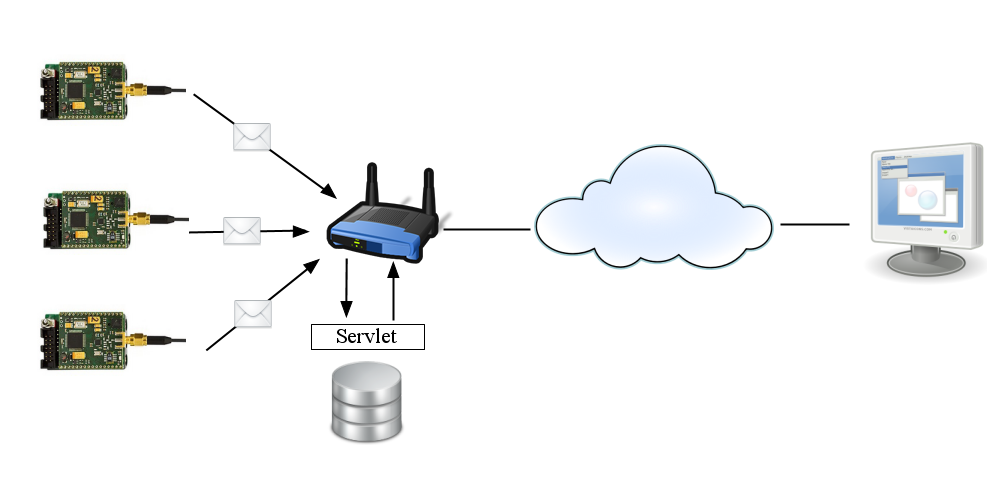
\includegraphics[width=12cm]{fig/Architektur.png}
   \caption{Architektur}
   \label{architecture}
\end{figure}

\section{Sensor-Knoten}
Der verwendete Sensor-Knoten basiert auf dem MSB430H-Board. Es enthält mehrere Sensoren. Diese sind der SHT11-Sensor , welcher die Temperatur und Luftfeuchtigkeit misst und der MMA 7260Q G-Sensor, 
mit dem die relative Lage des Sensor-Knotens im Raum festgestellt werden kann. Der Sensor-Knoten wurde mit dem WLAN-Modul RN-134 der Firma Roving Networks über die UART-Schnittstelle fest verlötet. 
Die Kommunikation zwischen dem programmierbaren Board und dem WLAN-Modul erfolgt also über die serielle Schnittstelle. An dieser Schnittstelle wurde ein Kipp-Schalter und  ein serielles Kabel angebracht, 
welche es ermöglichen, den Daten-Austausch zwischen Board und Modul zu verfolgen. Damit fiel das Debuggen der Kommunikation leichter.

\subsection{HTTP-Kommunikation}
Bei der Erprobung des WLAN-Moduls über eine serielle Schnittstelle haben wir verschiedene Übertragungsverfahren getestet: 

\begin{itemize}
 \item Das Modul bietet die Möglichkeit, alle x Sekunden einen UDP-Broadcast zu senden, welcher die auf dem Modul gesetzte Zeit beinhaltet und alle gemessenen Sensor-Werte. Dies ist für das Projekt nicht praktikabel, da die Sensoren nicht direkt an das WLAN-Modul angeschlossen sind, sondern an dem Sensor-Knoten. Deswegen ist auch der UDP-Unicast unbrauchbar.
 \item Das Modul bietet die Möglichkeit, eine TCP Auto-Connection zu nutzen, also automatisch alle x Sekunden aufzuwachen und eine TCP-Verbindung zu einem vordefinierten Host aufzurufen. Da das WLAN-Modul aber keine Werte vom Sensor-Knoten pollen kann, ist diese Methode ebenfalls unbrauchbar. 
 \item Eine weitere Methode, die aber ebenfalls wegen des oben beschriebenen Grundes fehlschlägt ist das automatische Senden von Sensor-Daten an einen HTTP-Server. 
\end{itemize}

Nach ausgiebigen Tests haben wir uns entschieden, die Daten über eine TCP-Verbindung zu verschicken. Diese wird von dem Sensor-Knoten geöffnet. Danach wird ein GET-Befehl des HTTP-Protokolls abgesetzt. Dabei wird angegeben, dass die Verbindung nicht geschlossen werden soll. Dies ermöglicht es (HTTP 1.1), mehrere Datensätze hintereinander mit Hilfe des GET-Befehls versendet, ohne die TCP-Verbindung jedes Mal neu initiieren zu müssen. Da die Verbindung nach ca. 5 Minuten vom Server geschlossen würde, muss sie in regelmäßigen Abständen vom Client geschlossen und direkt danach neu aufgebaut werden.  \\
Das WLAN-Modul verschickt einen festgelegten String (Default: „*HELLO* “), welcher nicht leer sein darf, beim erfolgreichen Aufbauen der TCP-Verbindung. Das hat uns zuerst Probleme bereitet hat, da der Tomcat-Server unbekannte Befehls-Präfices nicht ignoriert. Die Lösung ist das Benutzen von „GET“ als Communication-String. Da dieser aber nur beim Starten der Verbindung gesendet wird, muss jeder weitere GET-Befehl vollständig übertragen werden. Dies ist eine unschöne Lösung, allerdings lies sich das Problem nicht anders beheben, da das WLAN-Modul selbst nicht programmiert werden kann.

\subsection{Konfiguration des WLAN-Moduls}
Bei jedem Start des Sensor-Knotens muss das WLAN-Modul in einen wohldefinierten Zustand gebracht werden. Da beim Booten des Knotens nur schwer verifiziert werden kann, 
ob alle Einstellungen korrekt vorgenommen sind, haben wir uns dafür entschieden, dass das WLAN-Modul bei jedem Start auf die Fabrikeinstellungen  zurück gesetzt und dann neu konfiguriert wird. 
Dies ist nötig, da beim Programmieren der Sensor-Knoten zwar neu gestartet wurde beim Debuggen, die Stromversorgung des WLAN-Moduls aber nicht unterbrochen wurde und es so in einem beliebigen Zustand sein konnte. 
Das Zurücksetzen hat ebenfalls den Vorteil, dass das Modul nicht vor dem ersten Betrieb explizit initiiert werden muss, allerdings dauert jeder Boot-Vorgang etwas länger. Insgesamt jedoch werden bereits ca. 10 Sekunden nach dem Einschalten die ersten Sensor-Werte gesendet. 


\subsection{Programmierung des Sensor-Knotens}
Für die Programmierung des Sensor-Knotens wurde der Code Composer  [TODO: INSERT REAL NAME HERE] verwendet. Die Programmiersprache ist ein C-Dialekt, welcher fast alle Funktionen des Standards bereit stellt. \\
Das Programm des Sensor-Knotens besteht aus zwei Teilen: Zuerst wird eine Initalisierungs-Phase durchlaufen in der Interrupts angeschaltet werden, nötiger Speicher allociiert und das WLAN-Modul konfiguriert wird. Danach beginnt eine Endlos-Schleife, die das „Betriebssystem“ darstellt. 
In dieser Schleife werden die Sensor-Werte ermittelt und dann per WLAN verschickt.

\subsubsection{Initialisierung}
Bei der Initialisierung werden folgende Schritte chronologisch ausgeführt: 

\begin{itemize}
 \item Initialisierung der Port Register
 \item Aktivierung der quarzstabilen XT2 Taktquelle (7.3728MHz)
 \item Initialisierung der UART-RS232 Schnittstelle mit 9.6kBit/s
 \item Einschalten der Interrupts für die beiden Taster, Freigeben der Interrupts und  Aktivierung der Interrupt-Routinen
 \item Zurücksetzen des WLAN-Moduls in den Auslieferungszustand
 \item Setzen von WLAN-SSID, Passwort und anderen Parametern
 \item Verbindungsaufbau mit dem Access-Point und einrichten der TCP-Verbindung zum Tomcat-Server
\end{itemize}
Dann tritt das System in die zweite Phase ein.

\subsubsection{Betriebssystem}

Das „Betriebsystem“ besteht aus einer Endlos-Schleife, in der folgende Aktionen ausgeführt werden:
\begin{itemize}
 \item Überprüfung, ob bereits 20 Abfragen gesendet wurden; ggf. Trennung und erneuter Aufbau der TCP-Verbindung (der Server würde die Verbindung nach ca. 5 Minuten trennen)
 \item Auslesen der Sensoren, Aufbereitung der gelesenen Werte und Speicherung des Requests in einer Warteschlange, welche alle zu sendenden GET-Anfragen enthält
 \item Falls die Verbindung nicht gerade neu geöffnet wurde, wird „GET “ dem Request voran gestellt (Grund s.o.)  [REF EINFÜGEN]
 \item Solange noch weitere Requests in der Warteschlange sind, werden diese ebenfalls entfernt und dann versendet
\end{itemize}

\subsubsection{Tastendruck}
Die Erkennung eines Tastendrucks geschieht in dem in der Initialisierung definierten Interrupt. Dort wird direkt beim Interrupt und 0.5 Sekunden nach dem Auslösen gemessen, welcher Taster gedrückt wurde und dann beide Messungen logisch verodert. Damit können wir mit einem Interrupt ebenfalls feststellen, falls beide Taster gleichzeitig gedrückt wurden. Weiterhin kann damit ausgeschlossen werden, dass die analog gemessene Größe am Anfang noch etwas flackert und eventuell beim ersten Auslesen den falschen Wert liefert. Danach wird ein GET-Request für das Taster-Event erstellt und in die Warteschlange eingereiht. Beim nächsten Durchlauf der Betriebssystem-Schleife wird dieser Request dann ebenfalls mit verschickt. Die Auflösung der Tasten-Events ist damit gleich einem Schleifendurchlauf, der bei durchschnittlich 3 Sekunden, maximal bei 7 Sekunden (Trennen und neuer Aufbau der Verbindung) liegt. 

\section{Frontend}
Die Sensoren, die im Haushalt verteilt sind, schicken die gemessenen Daten an den Access Point. Nun müssen diese Daten in geeigneter Weise aufbereitet werden und den Nutzer zur Verfügung gestellt werden. Hierfür wurde eine Webseite gebaut, die es den Nutzer ermöglicht, die gemessenen Daten in Diagrammen darstellen zu lassen. \\
In diesem Kapitel wird dieses Frontend vorgestellt und beschrieben.

\subsection{Anforderungen}

An die Webseite, die es den Nutzer ermöglicht, die Daten der Sensoren zu überwachen, gibt es eine Reihe von Anforderungen. \\
Eine wichtige Anforderung ist die benutzerfreundliche Oberfläche, die in sich einfach gehalten ist und es den Anwender ermöglicht, sich schnell einzuarbeiten. Aus diesen Grund wurde die Oberfläche sehr schlicht gehalten und auf das Wesentliche reduziert.\\
Über eine Drop-down-Box kann der Nutzer zwischen den verschiedenen Sensoren auswählen und sich Daten anzeigen lassen. Dabei werden unterschiedliche Diagramme für die unterschiedlichen gemessenen Daten angezeigt. In unseren Fall hatten wir ein Diagramm für die Temperatur, Feuchtigkeit und 2 Diagramme für die Neigung des Sensors. Da es aber möglich sein soll, andere Sensoren an das System anzuschließen, welche andere Daten (Propertries) messen, passt sich die Oberfläche mit den Diagrammen an die jeweiligen Daten an. Es werden in die Diagramme angezeigt und mit Daten gefüllt, welche vom Sensor gemessen werden.\\
Nun kann der Nutzer die gemessene Werte überwachen. Dabei hat dieser aber nur ein Diagramm gleichzeitig im Blick (da pro Diagramm ein Tab in einem Tab-Menü zur Verfügung steht). Es kann passieren, dass der Anwender so zum Beispiel nicht beobachten kann, dass die Temperatur im Kühlschrank stetig zunimmt, weil dieser das Diagramm mit der Neigung des Sensors geöffnet hat. Damit der Nutzer gewarnt wird, wurden Trigger in unser System integriert. Dabei wird in serverseitiger und clientseitiger Trigger unterschieden. Wird eine Aktion auf der Clientseite ausgelöst, so wird eine Dialogbox auf der Webseite angezeigt. Wird eine serverseitige Aktion ausgelöst, so wird eine System-Ausgabe auf der Konsole ausgegeben.\\
Eine weitere Anforderung an das System war es, dass der Standort eines Sensors bearbeitet werden kann und dieser dann in die Datenbank abgespeichert wird. Es kann passieren, dass der mobile Sensorknoten an einen anderen Ort platziert wird. Bei der Anzeige der Sensordaten kann der Benutzer auf „Edit“ klicken und den Ort des Sensors bearbeiten. Die ID und die IP sollen nicht geändert werden. \\
Alle diese Anforderungen sind für die leichte Bedienbarkeit der Oberfläche und wurde in diesem System umgesetzt.

\section{Projekt zum Laufen bringen} \labelSec{abschnitt}

  
\section{Ausblick} \labelSec{ausblick}

\clearpage

\section{Appendix}

% @SETTINGS: Insert the name of your bibliography file WITHOUT extension.
\bibliography{main}

\bibliographystyle{abbrv}

\end{document}
